\documentclass[11pt,a4paper]{article}
\usepackage[spanish,es-nodecimaldot]{babel}	% Utilizar español
\usepackage[utf8]{inputenc}					% Caracteres UTF-8
\usepackage{graphicx}						% Imagenes
\usepackage[hidelinks]{hyperref}			% Poner enlaces sin marcarlos en rojo
\usepackage{fancyhdr}						% Modificar encabezados y pies de pagina
\usepackage{float}							% Insertar figuras
\usepackage[textwidth=390pt]{geometry}		% Anchura de la pagina
\usepackage[nottoc]{tocbibind}				% Referencias (no incluir num pagina indice en Indice)
\usepackage{enumitem}						% Permitir enumerate con distintos simbolos
\usepackage[T1]{fontenc}					% Usar textsc en sections
\usepackage{amsmath}						% Símbolos matemáticos
\usepackage[simplified]{pgf-umlcd}
\usepackage{pdflscape}
\usetikzlibrary{babel} % Problemas del español al usar <,> para las citas
\usepackage{typearea} % Paginas horizontales

\usepackage{listings}
\usepackage{xcolor}
 
\definecolor{codegreen}{rgb}{0,0.6,0}
\definecolor{codegray}{rgb}{0.5,0.5,0.5}
\definecolor{codepurple}{rgb}{0.58,0,0.82}
\definecolor{backcolour}{rgb}{0.95,0.95,0.92}
 
\lstdefinestyle{mystyle}{
    backgroundcolor=\color{backcolour},   
    commentstyle=\color{codegreen},
    keywordstyle=\color{magenta},
    numberstyle=\tiny\color{codegray},
    stringstyle=\color{codepurple},
    basicstyle=\ttfamily\footnotesize,
    breakatwhitespace=false,         
    breaklines=true,                 
    captionpos=b,                    
    keepspaces=true,                 
    numbers=left,                    
    numbersep=5pt,                  
    showspaces=false,                
    showstringspaces=false,
    showtabs=false,                  
    tabsize=4,
    language=Java
}
 
\lstset{style=mystyle}

% Comando para poner el nombre de la asignatura
\newcommand{\asignatura}{Nuevos Paradigmas de Interacción}
\newcommand{\autorv}{Vladislav Nikolov Vasilev}
\newcommand{\autorj}{José María Sánchez Guerrero}
\newcommand{\autorf}{Fernando Vallecillos Ruiz}
\newcommand{\titulo}{Práctica Sensores}
\newcommand{\subtitulo}{Memoria Técnica}


% Configuracion de encabezados y pies de pagina
\pagestyle{fancy}
\lhead{Vladislav, José María, Fernando}
\rhead{\asignatura{}}
\lfoot{Grado en Ingeniería Informática}
\cfoot{}
\rfoot{\thepage}
\renewcommand{\headrulewidth}{0.4pt}		% Linea cabeza de pagina
\renewcommand{\footrulewidth}{0.4pt}		% Linea pie de pagina


% new pagestyle
\fancypagestyle{lscape}{
  \headwidth\textwidth
}

\begin{document}
\pagenumbering{gobble}

% Pagina de titulo
\begin{titlepage}

\begin{minipage}{\textwidth}

\centering

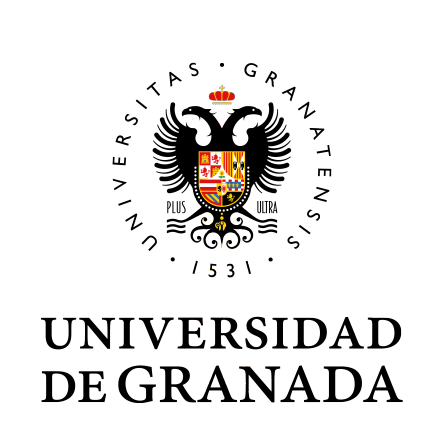
\includegraphics[scale=0.5]{img/ugr.png}\\

\textsc{\Large \asignatura{}\\[0.2cm]}
\textsc{GRADO EN INGENIERÍA INFORMÁTICA}\\[1cm]

\noindent\rule[-1ex]{\textwidth}{1pt}\\[1.5ex]
\textsc{{\Huge \titulo\\[0.5ex]}}
\textsc{{\Large \subtitulo\\}}
\noindent\rule[-1ex]{\textwidth}{2pt}\\[3.5ex]

\end{minipage}

\vspace{0.5cm}

\begin{minipage}{\textwidth}

\centering

\textbf{Autores}\\ {\autorv{}}\\{\autorj{}}\\{\autorf{}}\\[2.5ex]
\textbf{Rama}\\ {Computación y Sistemas Inteligentes}\\[2.5ex]
\vspace{0.3cm}


\includegraphics[scale=0.3]{img/etsiit.jpeg}

\vspace{0.5cm}
\textsc{Escuela Técnica Superior de Ingenierías Informática y de Telecomunicación}\\
\vspace{0.5cm}
\textsc{Curso 2019-2020}
\end{minipage}
\end{titlepage}

\pagenumbering{arabic}
\tableofcontents
\thispagestyle{empty}				% No usar estilo en la pagina de indice

\newpage

\setlength{\parskip}{1em}


\section{Introducción}
En este proyecto vamos a explicar nuestra \textit{Natural User Interface (NUI)} que hará que nuestra visita a la Alhambra sea más
dinámica y productiva. El proyecto constaría de varios dispositivos, como pueden ser principalmente unas gafas de realidad aumentada,
un dispositivo \textit{Leap Motion} y un micrófono integrados en las gafas, y un \textit{smartphone} que utilizaremos tanto para
manejar el sistema gracias a los múltiples sensores que incorpora como para controlar la aplicación.

En esta primera versión del proyecto vamos a encargarnos de la interfaz por sensores, es decir, dejaremos a un lado el \textit{Leap Motion}
y el controlador por voz. Vamos a encargarnos de la realidad aumentada y el resto de sensores para manejar el sistema.

\section{Interfaz por sensores}

Como no disponemos de unas gafas con estas características, simularemos su funcionamiento en la propia aplicación, utilizando un visor
VR con una imagen 3D del Patio de los Arrayanes y un lector de código QR. La idea es que estas dos características fuesen una sola, en
la cámara de las gafas. Por otro lado, llevaremos el \textit{smartphone} en la mano para controlar el contenido mostrado en las gafas, y
además, mostrará una maqueta de la Alhambra que nos servirá como mapa.

\subsection{Descripción del visor VR}
\label{sec:vr}

Por defecto, la aplicación lanza el \textbf{MainActivity} [\ref{sec:main}], inicializando la aplicación y mostrando el \textbf{ViewARFragment}
[\ref{sec:view}] (nuestro visor VR). El visor muestra una imagen de 360º, en la cual, cuando estemos mirando una estructura en concreto
(ya sea un edificio, puertas, columnas, jarrones, etc.), se nos marcará indicando que podremos interaccionar con ella.
Si movemos ligeramente el móvil hacia abajo cuando una de ellas esté resaltada, iniciamos la \textbf{InfoActivity} [\ref{sec:info}],
que es una pequeña página que muestra información extra sobre la estructura, como si fuese una enciclopedia. En nuestra aplicación esto
puede suponer un problema, ya que el visor lo tenemos en el móvil y al realizar el movimiento podemos deseleccionar lo que teníamos
resaltado; sin embargo, como esto estaría integrado en las gafas, cuando movamos el móvil, las gafas (que es donde vemos el objeto) no
se verán afectadas.

Una vez en el \textbf{InfoActivity}, para volver al visor VR, realizaremos un movimiento horizontal con nuestro dispositivo.
En nuestra aplicación, todo esto aparece en el dispositivo, pero en la versión definitiva, toda la información se mostraría en
las gafas.

\subsection{Descripción del lector QR}

En el menú desplegable, también tenemos la opción de \textit{Camera}, que nos lleva al \textbf{CameraFragment} [\ref{sec:camera}]. Este
implementa el lector de códigos QR, el cuál nos servirá a la hora de entrar a un edificio. Habrá códigos QR en cada uno y se obtendrá un
plano del edificio ya que las señales GPS pueden fallar o simplemente que el edificio tenga varias plantas y necesitemos ubicarnos mejor.
Cuando leamos un código se iniciará un \textbf{BlueprintsActivity}, que muestra la información anterior. Al igual que antes, para
volver a la cámara, realizaremos un movimiento horizontal con nuestro dispositivo.

\subsection{Descripción del mapa}
\label{sec:mapa}

Por último, en el menú desplegable tenemos un apartado llamado \textit{Navigation}, el cual inicia el
\textbf{NavigationFragment} [\ref{sec:nav}]
que nos muestra un maquetado 3D de toda la Alhambra con regiones clickables señaladas para saber en que lugar nos encontramos o si queremos
ir a algún otro lugar. Esta parte será la única que se vea en el \textit{smartphone}. Tendremos implementados en él, el siguiente multitouch:

\begin{itemize}
    \item \textbf{Click simple}. Servirá para seleccionar y deseleccionar las regiones clickables.
    \item \textbf{Click simple arrastable}. Nos permite desplazarnos por el mapa.
    \item \textbf{Doble click}. Hacemos zoom en el mapa un valor predeterminado.
    \item \textbf{Pellizcar}. Ampliamos y alejamos la zona del mapa, dependiendo de hacia donde pellizquemos.
    \item \textbf{Click con dos dedos y arrastre}. Entramos en el modo 3D del mapa. En él nos desplazaremos como acabamos de ver.
    \item \textbf{Click con dos dedos y rotación}. Estando en el modo 3D, esto nos servirá para rotar la vista alrededor de la maqueta.
\end{itemize}

Como podemos ver, utilizamos bastantes sensores multitouch, pero no hay ninguno que requiera del acelerómetro, giroscopio, etc., por lo
que no tendremos colisiones entre éste y los mencionados anteriormente.



% start new page before setting page layout,
% otherwise previous page is also affected
\KOMAoption{paper}{landscape}%
\typearea{12}% sets new DIV

% Establecer pagina horizontal
\recalctypearea
% needed to show page in landscape in viewer
\pdfpageheight=\paperheight
\pdfpagewidth=\paperwidth
% Poner estilo
\pagestyle{lscape}

\newpage

\section{Diagrama de clases}

A continuación se puede ver el diagrama de clases. No se han incluido atributos ni métodos porque se van a describir más adelante.

\begin{figure}[H]
\centering
\begin{tikzpicture}[scale=0.7]
	\begin{class}[text width=3cm]{MainActivity}{0,0}
	\end{class}
	
	\begin{class}[text width=4cm]{CameraFragment}{-9, -5}
	\end{class}
	\begin{class}[text width=3cm]{ExitFragment}{-7, -1}
	\end{class}
	\begin{class}[text width=5cm]{NavigationFragment}{0, -6.5}
	\end{class}
	\begin{class}[text width=4cm]{ViewARFragment}{9, -5}
	\end{class}
	\begin{class}[text width=4cm]{BlueprintsActivity}{-9, -9}
	\end{class}
	\begin{class}[text width=3cm]{InfoActivity}{9, -9}
	\end{class}
	
	\unidirectionalAssociation{MainActivity}{}{1}{CameraFragment}
	\unidirectionalAssociation{MainActivity}{}{1}{ExitFragment}
	\unidirectionalAssociation{MainActivity}{}{1}{NavigationFragment}
	\unidirectionalAssociation{MainActivity}{}{1}{ViewARFragment}
	
	\draw[umlcd style dashed line,->] (ViewARFragment) -- node[above, sloped, black] {$<<$uses$>>$} (InfoActivity);
	\draw[umlcd style dashed line,->] (CameraFragment) -- node[above, sloped, black] {$<<$uses$>>$} (BlueprintsActivity);
\end{tikzpicture}
\caption{Diagrama de clases simplificado.}
\label{fig:class-diagram}
\end{figure}

\KOMAoptions{paper=portrait}
\recalctypearea
\pdfpageheight=\paperheight
\pdfpagewidth=\paperwidth
\headwidth\textwidth

\section{Descripción de las clases}

Una vez visto el diagrama de clases, vamos a proceder a comentar brevemente qué es lo que hace cada clase, sus
atributos, y sus métodos.

\subsection{\textbf{MainActivity}}
\label{sec:main}

Es la actividad principal, encargada de construir la barra de actividades que permite acceder
a los \textit{fragments} y de solicitar los permisos de cámara y localización necesarios para ejecutar
la aplicación.

\subsubsection{Atributos}

Los atributos que tiene esta clase son los siguientes:

\begin{itemize}
    \item \textit{mAppBarConfiguration}: Esta variable contiene la barra de navegación, con las distintas opciones que ofrece (navegación,
    VR, etc.).
    \item \textit{\textbf{PERMISSION\_ALL}}: Código de permiso usado cuando se piden los permisos. Su valor da igual, pero tiene que ser mayor
    o igual a 0, según la documentación de Android \cite{bib:permisos}. En este caso, se le ha asignado el valor 1.
    \item \textit{\textbf{PERMISSIONS}}: Array con los permisos a pedir (localización y cámara).
\end{itemize}

\subsubsection{Métodos}

El siguiente método comprueba si se tienen los permisos necesarios (según los que se hayan especificado en \textit{\textbf{PERMISSIONS}}).
Si están todos, devuelve \textbf{true}. En caso contrario, devuelve \textbf{false}.

\begin{lstlisting}
private boolean hasPermisions() { ... }
\end{lstlisting}

El siguiente método inicializa la barra de navegación y solicita los permisos necesarios, si se tiene que hacer. Sobreescribe al método
de la superclase. El parámetro serviría para restaurar información, de ser necesario.

\begin{lstlisting}
protected void onCreate(Bundle savedInstanceState) { ... }
\end{lstlisting}

El siguiente método se llama al crear el menú (la barra de navegación, en este caso) la primera vez. Devuelve siempre \textbf{true}.

\begin{lstlisting}
public boolean onCreateOptionsMenu(Menu menu) { return true; }
\end{lstlisting}

El siguiente método se llama cuando se despliega la barra de navegación, y devuelve \textbf{true} si se ha podido desplegar
correctamente, y \textbf{false} en caso contrario. Sobreescribe al método de la superclase.

\begin{lstlisting}
public boolean onSupportNavigateUp() { ... }
\end{lstlisting}

\subsection{\textbf{ExitFragment}}
\label{sec:exit}

\textit{Fragment} que pregunta al usuario si quiere salir o no de la aplicación y, en caso afirmativo, la cierra.

\subsubsection{Atributos}

Esta clase no dispone de atributos, ya que no necesita guardar ningún tipo de información.

\subsubsection{Métodos}

El siguiente método es llamado cuando se crea la vista. Crea un cuadro de diálogo donde pregunta al usuario si quiere o no salir de la
aplicación. En caso afirmativo, la cierra. En caso contrario, no hace nada y cierra el diálogo. Los atributos pasados son los típicos
a la hora de crear una vista de un \textit{fragment} \cite{bib:fragment}.

\begin{lstlisting}
public View onCreateView(@NonNull LayoutInflater inflater,
                         ViewGroup container,
                         Bundle savedInstanceState) { ... }
\end{lstlisting}

\subsection{\textbf{CameraFragment}}
\label{sec:camera}

\textit{Fragment} que permite acceder al sensor de la cámara para poder realizar la lectura
de códigos QR. Una vez leídos, se encarga también de pasarlos a \textbf{BlueprintActivity} para que éste los procese.
Para la detección y lectura de los códigos QR se utiliza la biblioteca \textit{BarcodeDetector}.

\subsubsection{Atributos}

La clase dispone de los siguientes atributos:

\begin{itemize}
    \item \textit{surfaceView}: Superficie donde se mostrará la cámara.
    \item \textit{cameraSource}: Se encarga de recibir la información de la cámara y de mandársela al lector de códigos QR.
    \item \textit{barcodeDetector}: Detector de códigos QR que se va a utilizar.
    \item \textit{lecturaQR}: Contiene la información de lo que ha leído el lector de QR en formato String. Se utilizará para
    determinar que información mostrar en función del valor que tenga guardado.
\end{itemize}

\subsubsection{Métodos}

El siguiente método se llama al crear la vista donde se mostrará lo que vaya viendo la cámara. Se usa un \textbf{SurfaceView} para mostrar
la imagen de manera más rápida. Los parámetros son los mismos que en el caso de \textbf{ExitFragment}. Para obtener más información
sobre estos, se puede consultar la misma referencia que en ese caso.

\begin{lstlisting}
public View onCreateView(@NonNull LayoutInflater inflater,
                         ViewGroup container,
                         Bundle savedInstanceState) { ... }
\end{lstlisting}

El siguiente método se llama cuando se pausa la actividad del \textit{fragment}. Llama al método de la superclase.

\begin{lstlisting}
public void onPause() { ... }
\end{lstlisting}

El siguiente método se llama cuando se reanuda la actividad del \textit{fragment}. Llama al método de la superclase y a
\textit{activateCameraReader()} para activar la cámara.

\begin{lstlisting}
public void onResume() { ... }
\end{lstlisting}

El siguiente método se llama cuando se destruye la actividad. Llama al método de la superclase.

\begin{lstlisting}
public void onDestroy() { ... }
\end{lstlisting}

El siguiente método es llamado cuando se reanuda la actividad. Activa la cámara, establece cómo se tiene que manejar la información
que le llegue a ésta utilizando para ello las variables \textit{barcodeDetector} y \textit{cameraSource} y crea una vista donde se podrá
ver la imagen que esté procesando la cámara, utilizando para ello \textit{surfaceView}. Establece además que cuando se detecte un
código QR se pare la cámara, dejando de recibir información nueva, y que se lance una \textbf{BlueprintsActivity} para determinar qué mostrar
en función del primer valor leído. Después de este procesamiento, se limpia la lista de QR leídos.

\begin{lstlisting}
public void activateCameraReader() { ... }
\end{lstlisting}

\subsection{\textbf{NavigationFragment}}
\label{sec:nav}

\textit{Fragment} que permite acceder a un mapa de la Alhambra y navegar por él, destacando
algunos de los edificios y permitiendo interactuar con ellos, tal y como se ha descrito en la sección \ref{sec:mapa}.
Para poder trabajar con mapas, se utiliza la API de GoogleMaps.

\subsubsection{Atributos}

Los atributos de la clase son los siguientes:

\begin{itemize}
    \item \textit{googleApiClient}: Cliente de la API de Google.
    \item \textit{\textbf{MIN\_CAMBIO\_DISTANCIA\_PARA\_UPDATES}}: Mínima distancia que se debe haber recorrido para que se realice una
    actualización del marcador de posición actual. Se ha establecido que sean 10 metros.
    \item \textit{\textbf{MIN\_TIEMPO\_ENTRE\_UPDATES}}: Mínimo tiempo que debe transcurrir para que se actualice el marcador de
    la posición actual. El tiempo viene dado en milisegundos. Se ha establecido que sean 5000 milisegundos, es decir, unos 5 segundos.
    \item \textit{nMap}: Mapa de Google que se mostrará  sobre el que se crearán las zonas destacadas y se mostrará la posición del
    dispositivo.
    \item \textit{image}: Imagen que se mostrará al pulsar sobre una zona destacada.
    \item \textit{locListener}: \textit{Listener} que se usará para actualizar la posición actual del dispositivo en el mapa.
\end{itemize}

\subsubsection{Métodos}

El siguiente método se lanza al crear la vista. Establece una conexión con la API de Google para poder utilizar sus servicios más adelante.
Además, carga la \textit{ImageView} donde se mostrarán las imágenes de las zonas destacadas al pulsar sobre ellas, poniéndola invisible
de momento.

\begin{lstlisting}
public View onCreateView(@NonNull LayoutInflater inflater,
                         ViewGroup container,
                         Bundle savedInstanceState) { ... }
\end{lstlisting}

El siguiente método se lanza cuando el mapa está listo. Recibe como parámetro el mapa de Google, el cuál se asigna a \textit{nMap}. Establece
un estilo personalizado que utilizará el mapa, además de ponerle unos límites para que esté más o menos centrado en la Alhambra y para que
no se pueda salir de éste, y establece un zoom inicial, el cuál será el máximo \textit{zoom out} que se pueda hacer. Además, crea las
zonas destacadas sobre el mapa, las pone visibles y establece qué imagen se debe mostrar al pulsar sobre cada una de ellas. Finalmente,
establece cómo se debe realizar la actualización de la posición actual, utilizando para ello \textit{locListener} y los
atributos de distancia mínima y tiempo mínimo.

\begin{lstlisting}
public void onMapReady(GoogleMap googleMap) { ... }
\end{lstlisting}

El siguiente método se lanza cuando se establece la conexión con la API de Google. No se hace nada.

\begin{lstlisting}
public void onConnected(@Nullable Bundle bundle) { }
\end{lstlisting}

El siguiente método se lanza cuando se suspende la conexión con la API de Google. No se hace nada.

\begin{lstlisting}
public void onConnectionSuspended(int i) { }
\end{lstlisting}

El siguiente método se lanza cuando falla la conexión con la API de Google. No se hace nada.

\begin{lstlisting}
public void onConnectionFailed(@NonNull ConnectionResult connectionResult) { }
\end{lstlisting}

\subsection{\textbf{ViewARFragment}}
\label{sec:view}

\textit{Fragment} que simula la visión en realidad aumentada del interior de los Palacios
Nazaríes. Simula que detecta zonas interesantes y las destaca. Cuando se realiza un gesto con el dispositivo, tal y como se
ha indicado en la sección \ref{sec:vr}, muestra más información sobre el elemento destacado, utilizando para ello la clase
\textbf{InfoActivity}.

\subsubsection{Atributos}

Los atributos de los que dispone la clase son los siguiente:

\begin{itemize}
    \item \textit{imagen}: Imagen a mostrar en cada momento.
    \item \textit{mVRPanoramaView}: VR asociado a la imagen correspondiente.
    \item \textit{sensorManager}: Gestor de sensores. Permite acceder a los distintos sensores, aunque nos interesa el acelerómetro.
    \item \textit{mHeadRotation}: Rotación de la cabeza en grados.
    \item \textit{lastUpdate}: Último instante en el que se ha actualizado el sensor.
    \item \textit{last\_y}: Último valor de Y registrado con el acelerómetro.
    \item \textit{\textbf{SHAKE\_THRESHOLD}}: Umbral del acelerómetro. Se reconoce el gesto del \textit{shake} cuando la aceleración
    del acelerómetro supera este umbral, el cuál es de 200.
    \item \textit{\textbf{UPDATE\_TIME\_THRESHOLD}}: Tiempo mínimo entre actualizaciones del acelerómetro en milisegundos. Es decir,
    no se van a tener en cuenta aquellas actualizaciones que se hagan con un margen de tiempo demasiado pequeño. Se ha establecido
    que sean 250 milisegundos.
\end{itemize}

\subsubsection{Métodos}

El siguiente método se llama cuando se crea la vista. Se carga el gesetor de sensores, la imagen inicial del VR y se obtiene la rotación
inicial de la cabeza.

\begin{lstlisting}
public View onCreateView(@NonNull LayoutInflater inflater,
                         ViewGroup container,
                         Bundle savedInstanceState) { ... }
\end{lstlisting}

El siguiente método se llama cuando se pausa la actividad. Se pasa la renderización del VR y se detiene el registro de los sensores.

\begin{lstlisting}
public void onPause() { ... }
\end{lstlisting}

El siguiente método se llama cuando se reanuda la actividad. La renderización del VR continua y se comienza a registrar la actividad
del acelerómetro.

\begin{lstlisting}
public void onResume() { ... }
\end{lstlisting}

El siguiente método se llama cuando se destruye la actividad. Apaga la renderización del VR.

\begin{lstlisting}
public void onDestroy() { ... }
\end{lstlisting}

El siguiente método carga la imagen actual en el VR. En caso de que se produzca algún error, se muestra información de depuración.

\begin{lstlisting}
private void loadPhotoSphere() { ... }
\end{lstlisting}

El siguiente método se llama si se cambia la precisión de los sensores. Se le debe hacer un \textit{override} ya que la clase
implementa la interfaz \textbf{SensorEventListener}. No se realiza ninguna acción.

\begin{lstlisting}
public void onAccuracyChanged(Sensor sensor, int accuracy) { ... }
\end{lstlisting}

El siguiente método se llama cuando se produce algún cambio en alguno de los sensores. Recibe como parámetro un evento provocado
por algún sensor. Si el evento es provocado por el acelerómetro, ha pasado tiempo suficiente desde la última actualización y se ha
superado la aceleración umbral, se lanza un \textit{intent} con la clase \textbf{InfoActivity} para mostrar información sobre las
regiones destacadas y se actualizan los valores de \textit{lastUpdate} y \textit{last\_y}. En cualquier caso, se produzca el evento
que se produzca, se actualiza la rotación de la cabeza y se mira si se tiene que actualizar la imagen que se está mostrando llamando
para ello a \textit{updateReticule()}.

\begin{lstlisting}
public void onSensorChanged(SensorEvent sensorEvent) { ... }
\end{lstlisting}

El siguiente método actualiza la imagen que se está mostrando en el VR en función de la rotación de la cabeza que se ha obtenido en
\textit{onSensorChanged()}.

\begin{lstlisting}
private void updateReticule() { ... }
\end{lstlisting}

\subsection{\textbf{BlueprintsActivity}}
\label{sec:blue}

Actividad que se encarga de recibir las lecturas QR de \textbf{CameraFragment} y de procesarlas, mostrando la información
correspondiente a la lectura.

\subsubsection{Atributos}
Los atributos presentes en esta clase son los siguientes:

\begin{itemize}
    \item \textit{tituloPlano}: \textbf{TextView} del título del plano que se va a mostrar en la vista.
    \item \textit{plantaPlano}: \textbf{TextView} con la información sobre la planta o localización.
    \item \textit{imagenPlano}: \textbf{ImageView} con la imagen que se mostrará. En este caso, es una imagen de un plano con o
    sin una localización marcada.
    \item \textit{sensorManager}: Gestor de sensores. Permite acceder a los distintos sensores, aunque nos interesa el acelerómetro.
    \item \textit{senAccelerometer}: Acelerómetro.
    \item \textit{lastUpdate}: Último instante en el que se ha actualizado el sensor.
    \item \textit{last\_x}: Último valor de X registrado con el acelerómetro.
    \item \textit{\textbf{SHAKE\_THRESHOLD}}: Umbral del acelerómetro. Se reconoce el gesto del \textit{shake} cuando la aceleración
    del acelerómetro supera este umbral, el cuál es de 200.
    \item \textit{\textbf{UPDATE\_TIME\_THRESHOLD}}: Tiempo mínimo entre actualizaciones del acelerómetro en milisegundos. Es decir,
    no se van a tener en cuenta aquellas actualizaciones que se hagan con un margen de tiempo demasiado pequeño. Se ha establecido
    que sean 200 milisegundos.
\end{itemize}

\subsubsection{Métodos}

El siguiente método se llama cuando se crea la actividad. Determina qué información debe mostrar en función de lo que indique
la variable \textit{lecturaQr} de la clase \textbf{CameraFragment}. Además de eso, inicializa el gestor de sensores y la detección
del acelerómetro.

\begin{lstlisting}
protected void onCreate(Bundle savedInstanceState) { ... }
\end{lstlisting}

El siguiente método se llama para mostrar la vista que contiene el título, el plano y la información sobre el plano. Recibe como entrada
el nombre del archivo con la imagen del plano correspondiente, el texto del título y el texto de información.

\begin{lstlisting}
private void showImageTextInfo(String fileName, String title, String information) { ... }
\end{lstlisting}

El siguiente método se llama cuando se produce algún cambio en alguno de los sensores. Recibe como parámetro un evento provocado
por algún sensor. Si el evento es provocado por el acelerómetro, ha pasado tiempo suficiente desde la última actualización y se ha
superado la aceleración umbral, se finaliza la tarea actual para volver a la que estábamos anteriormente y se actualizan los valores de \textit{lastUpdate} y \textit{last\_x}.

\begin{lstlisting}
public void onSensorChanged(SensorEvent sensorEvent) { ... }
\end{lstlisting}

El siguiente método se llama si se cambia la precisión de los sensores. Se le debe hacer un \textit{override} ya que la clase
implementa la interfaz \textbf{SensorEventListener}. No se realiza ninguna acción.

\begin{lstlisting}
public void onAccuracyChanged(Sensor sensor, int accuracy) { ... }
\end{lstlisting}

\subsection{\textbf{InfoActivity}}
\label{sec:info}

Actividad que muestra información sobre la zona que ha sido destacada en \textbf{ViewARFragment}.
Procesa la información que tiene ésta y muestra una u otra información.

\subsubsection{Atributos}

Esta clase tiene los siguientes atributos:

\begin{itemize}
    \item \textit{tituloInfo}: \textbf{TextView} del título de lo que se quiere mostrar.
    \item \textit{textInfo}: \textbf{TextView} con la información de lo que se quiere mostrar.
    \item \textit{imageView}: \textbf{ImageView} con la imagen que se mostrará de alguna de las regiones destacadas.
    \item \textit{sensorManager}: Gestor de sensores. Permite acceder a los distintos sensores, aunque nos interesa el acelerómetro.
    \item \textit{senAccelerometer}: Acelerómetro.
    \item \textit{lastUpdate}: Último instante en el que se ha actualizado el sensor.
    \item \textit{last\_x}: Último valor de X registrado con el acelerómetro.
    \item \textit{\textbf{SHAKE\_THRESHOLD}}: Umbral del acelerómetro. Se reconoce el gesto del \textit{shake} cuando la aceleración
    del acelerómetro supera este umbral, el cuál es de 200.
    \item \textit{\textbf{UPDATE\_TIME\_THRESHOLD}}: Tiempo mínimo entre actualizaciones del acelerómetro en milisegundos. Es decir,
    no se van a tener en cuenta aquellas actualizaciones que se hagan con un margen de tiempo demasiado pequeño. Se ha establecido
    que sean 200 milisegundos.
\end{itemize}

\subsubsection{Métodos}

El siguiente método se llama cuando se crea la actividad. Inicializa el gestor de sensores y la detección del acelerómetro y muestra
la vista correspondiente en función del atributo \textit{imagen} de la clase \textbf{ViewARFragment}.

\begin{lstlisting}
protected void onCreate(Bundle savedInstanceState) { ... }
\end{lstlisting}

El siguiente método se llama cuando se produce algún cambio en alguno de los sensores. Recibe como parámetro un evento provocado
por algún sensor. Si el evento es provocado por el acelerómetro, ha pasado tiempo suficiente desde la última actualización y se ha
superado la aceleración umbral, se finaliza la tarea actual para volver a la que estábamos anteriormente y se actualizan los valores de \textit{lastUpdate} y \textit{last\_x}.

\begin{lstlisting}
public void onSensorChanged(SensorEvent sensorEvent) { ... }
\end{lstlisting}

El siguiente método se llama cuando se pausa la actividad. Se le indica al gestor de sensores que deje recibir información.

\begin{lstlisting}
public void onPause() { ... }
\end{lstlisting}

El siguiente método se llama cuando se reanuda la actividad. Se vuelve a registrar el acelerómetro.

\begin{lstlisting}
public void onResume() { ... }
\end{lstlisting}

El siguiente método se llama cuando se destruye la actividad. Llama al método de la superclase.

\begin{lstlisting}
public void onDestroy() { ... }
\end{lstlisting}

El siguiente método se llama si se cambia la precisión de los sensores. Se le debe hacer un \textit{override} ya que la clase
implementa la interfaz \textbf{SensorEventListener}. No se realiza ninguna acción.

\begin{lstlisting}
public void onAccuracyChanged(Sensor sensor, int accuracy) { ... }
\end{lstlisting}

\newpage

\begin{thebibliography}{5}

\bibitem{bib:permisos}
Permisos en Android
\\\url{https://developer.android.com/reference/androidx/core/app/ActivityCompat.html#requestPermissions(android.app.Activity,%20java.lang.String%5B%5D,%20int)}

\bibitem{bib:fragment}
\textit{Fragment} en Android
\\\url{https://developer.android.com/reference/android/app/Fragment#onCreateView(android.view.LayoutInflater,%20android.view.ViewGroup,%20android.os.Bundle)}

\end{thebibliography}

\end{document}

